
\def \Subject {تمرین اول}
\def \Author {رامتین احسانی }
\def \Date {1400/7/23}
\def \Session {1}
\setcounter{chapter}{\Session-1}

\chapter{\Subject}
\chapterauthor{\Author~ - \Date}

تمرین اول
درس 
\CourseName  
 تهیه شده توسط
\Author
 با استفاده از سیستم حروف چینی
\grayBox {LaTeX} 
و بسته ی 
\grayBox{XePersian}


\section{در حال حاضر تا چه میزان می توان در یک زمان معقول حمله Brute-force انجام داد؟}
میدانیم که از 
\grayBox{Brute-force attack}
برای حمله به سیستم ها برای شکستن رمز آن ها و دسترسی
\textbf{غیر مجاز}
به آن ها استفاده میشود.
در این نوع حمله تمام حالت های ممکن فضای کلید را امتحان میکنیم تا بالاخره کلید درست را پیدا کنیم.
انواع مختلفی از این نوع حمله وجود دارد مانند:
\begin{itemize}
    \item    
    attack force brute Simple   
    \item
    attacks Dictionary
    \item
    attack force brute Reverse
    \item
    ...
\end{itemize}
\subsection{میزان درصد حمله های Brute-force}
در کل،
طبق اطلاعات ثبت شده از حمله های سایبری تایید شده
چیزی حدود 
\textbf{5 درصد}
از حمله ها از نوع
Brute-force 
هستند.
در صورت استفاده از این روش به احتمال 1 به 5 احتمالا موفق خواهید شد.

\subsection{سرعت}
سرعت شکستن رمز با استفاده از 
Brute-force
به دو چیز بستگی دارد:

\begin{itemize}
    \item    
    قدرت رمز سیستم هدف
    \item
    قدرت سیستم حمله کننده
\end{itemize}
در کل سیستم های حمله کننده میتوانند چیزی حدود 
\textbf{10,000}
تا 
\textbf{1 بیلیون}
رمز در ثانیه را تست کنند.
یک سیستم با سخت افزار 
\grayBox{Pentium 100}
میتواند 10 هزار رمز را در ثانیه چک کتد.
در حالی که یک سوپر کامپیوتر با سخت افزار های قوی میتواند تا 1 بیلیون رمز را در ثانیه امتحان کند.
\begin{itemize}
    \item    
    چیزی حدود 94 کاراکتر در یک کیبورد استاندارد وجود دارد که در کل میتوانند 2 بیلیون رمز 8 کاراکتری به وجود بیاورند.
    \item
    هر چقدر این رمز ها رندوم تر و پیچیده تر باشند، شکستن آن ها سخت تر میشود. یک رمز با طول 9 با کاراکتر های متفاوت چیزی حدود 2 ساعت طول میکشد تا شکسته شود. اگر کاراکتر ها یکسان باشند چیزی حدود 2 دقیقه طول میکشد.
    \item
    یک رمز با 12 کاراکتر متفاوت به 3 قرن زمان احتیاج دارد تا شکسته شود!
    \item
    یک کلید با 
    \textbf{256-bit}،
    \lr{2$^{256}$}
    حالت مختلف برای حمله کننده ایجاد میکند که شکستن آن به 
    \textbf{تریلیون}
    سال ها احتیاج دارد.
\end{itemize}
یک رمز ساده حاوی کاراکتر های 
\textbf{lowercase}
در سیستمی حاوی 
\grayBox{Pentium 100}
در 5.8 ساعت شکسته میشود 
و در یک سوپر کامپیوتر این اتفاق با سرعت بسیار زیادتر و تقریبا بلافاصله صورت میگیرد.
با افزایش طول رمز، زمان لازم برای شکستن آن به صورت 
\textbf{نمایی}
بیشتر میشود.

\section{انواع رمزهای جانشینی}
در این نوع از رمزگذاری، جایگاه حروف در یک متن بهم نمی خورد، تنها هر حرف یا گروهی از حروف با یک
حرف یا گروهی دیگر از حروف جابجا می شوند.
در این گزارش انواع این رمز ها را معرفی میکنم.
\subsection{\lr{Mono-alphabetic Cipher}}
انواع:
\begin{itemize}
    \item   
    \lr{Atbash Cipher}
    \item
    \lr{ROT13 Cipher}
    \item
    \lr{Caesar Cipher}
    \item
    \lr{Affine Cipher}
    \item
    \lr{Baconian Cipher}
    \item
    \lr{Polybius Square Cipher}
    \item
    \lr{Simple Substitution Cipher}
    \item
    \lr{Codes and Nomenclators Cipher}
\end{itemize}
برای مثال، الگوریتم 
\grayBox{ROT13} 
همان الگوریتم سزار با شیفت 13 است.
این الگوریتم ها بخاطر سادگی که دارند در جاهای حساس استفاده خاصی ندارند و بیشتر در 
\grayBox{Online Forum} ها
برای مخفی کردن متن ها استفاده میشوند.
\subsection{\lr{Homophonic Substitution Cipher}}
انواع:
\begin{itemize}
    \item   
    \lr{Beale ciphers}
\end{itemize}
این نوع الگوریتم ها مانند 
\grayBox{Mono-alphabetic Cipher} 
هستند با این تفاوت که یک حرف به چند حرف تبدیل میشود.
\grayBox{Beale ciphers} 
یک نوع از این الگوریتم ها است که مکان یک گنج را در داخل 3 متن مخفی کرده است.

\subsection{\lr{Polygram Substitution Cipher}}
در این نوع از سایفر، بلوکی از کلمات با بلوکی از کلمات دیگر جایگزین میشوند.
\begin{figure}[H]
    \centering
    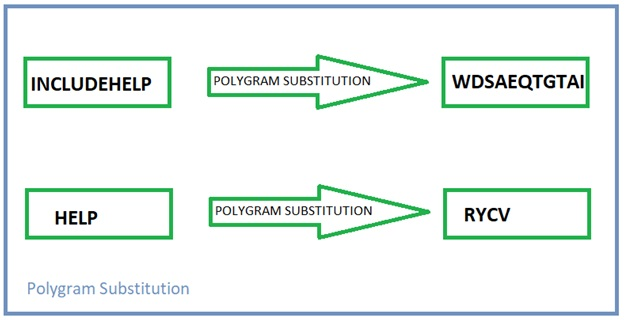
\includegraphics[width=0.5\linewidth]{images/substitution.jpg}
    \caption{\lr{Polygram Substitution Cipher}}
    \label{fig:Polygram}
\end{figure}
انواع:
\begin{itemize}
    \item   
    \lr{Four-Square Cipher}
    \item
    \lr{Hill Cipher}
    \item
    \lr{Caesar Cipher}
    \item
    \lr{Playfair Cipher}
\end{itemize}
بریتانیا از الگوریتم 
\grayBox{Playfair cipher} 
در جنگ جهانی اول استفاده کرد.

\subsection{\lr{Polyalphabetic Substitution Cipher}}
همانطور که از اسم مشخص است این الگوریتم ها چند الفبایی هستند.
انواع:
\begin{itemize}
    \item   
    \lr{Autokey Cipher}
    \item
    \lr{Beaufort Cipher}
    \item
    \lr{Porta Cipher}
    \item
    \lr{Running Key Cipher}
    \item
    \lr{Enigma Cipher}
    \item
    \lr{Vigenère and Gronsfeld Cipher}
\end{itemize}
الگوریتم ویگنر را در کلاس بررسی کردیم. الگوریتم 
\grayBox{Autokey cipher} 
فرقی کوچکی با ویگنر دارد که وقتی کلید مشخص شد،
برای رمزگشایی از خود PlainText هم در کلید استفاده میکنیم.
مثال:
کلید ما 
\textbf{FORTIFICATION}
است.
\begin{figure}[H]
    \centering
    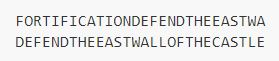
\includegraphics[width=0.5\linewidth]{images/auto.JPG}
    \caption{\lr{Autokey Cipher}}
    \label{fig:Polygram}
\end{figure}

با تشکر، تهیه شده توسط رامتین احسانی
\nocite{*}
